\documentclass[french]{template}

\begin{document}

\titre{Projet Newtonoid}
\UE{Programmation Fonctionnelle}
\enseignant{Guilaume \textsc{Dupont}}
\eleves{Romain \textsc{Haessler} \\ Benjamin \textsc{Pascal} \\ Leïlie \textsc{Canillac} \\ Vianney \textsc{Hervy}}

\fairemarges
\fairepagedegarde
\tabledematieres

\newpage

\section{Introduction}

\section{Architecture}

Les sources sont réparties en deux répertoires: \texttt{bin} et \texttt{lib}.

\begin{itemize}
    \item \texttt{bin} contient le programme principal \texttt{newtonoid.ml} qui peut utiliser les modules de la bibliothèque \texttt{Libnewtonoid}.
    \item \texttt{lib} contient les modules et interfaces impémentant les divers éléments du jeu. Le fichier \texttt{lib/dune} contient une directive pour créer une bibliothèque appelée \texttt{Libnewtonoid} contenant tous les modules de \texttt{lib}.
\end{itemize}

Les répertoires \texttt{configs} et \texttt{levels} contiennent respectivement des configuration et des niveaux d'exemple.

\subsection{Modules}

La plupart des modules de \texttt{Libnewtonoid} sont dotés d'une interface documentée en \texttt{.mli}. Certains modules sont relatifs à des objets: \texttt{Ball}, \texttt{Box}, \texttt{Brick}, \texttt{Level}, \texttt{Paddle}, \texttt{State}. Tandis que d'autres sont un groupement de fonctions nécessaires à une fonctionnalité: \texttt{Collision}, \texttt{Input}, \texttt{Iterator}, \texttt{LoadLevel}, \texttt{Utils}, \texttt{ParamValidator}, \texttt{Iterator}.

La plupart des modules contiennent un sous-module foncteur (au sens d'OCaml) paramétré par un module \texttt{P}. On a donc une structure récurrente de la forme: \texttt{module Make(P: Params)} qui permet d'instancier le foncteur avec les paramètres fournis par l'utilisateur.

\section{Objets}

Chaque objet du jeu est modélisé par un type enregistrement afin de permettre un accès efficace aux différents champs (par opposition aux tuples qui nécessitent du filtrage par motif). Chaque type objet est appelé \texttt{t} et est défini dans son propre module qui regroupe les fonctions associées. Parmis celles-ci, on note surtout \texttt{make}, \texttt{draw} et \texttt{draw\_shadow} et qui permettent respectivement de créer un objet, de l'afficher à l'écran et de dessiner son ombre.

\section{États de jeu}

Au lancement du jeu, notre système est à l'état initial (Init). En effectuant un clique de souris, notre jeu pass à l'état Playing. Si l'on clique à nouveau cela nous permet de mettre le jeu en pause. En jouant la partie, il y a trois façons de sortir de l'état Playing :

\begin{itemize}
    \item Si l'on réussit à casser toutes les briques, le niveau est alors fini. On passe à l'état Victory. En cliquant a nouveau on passe au niveau suivant. Si tous les niveaux sont terminés, le jeu s'arrête.
    \item Si on perd une vie sans tomber à 0, le jeu retourne à l'état initial mais avec une vie en moins. Pour reprendre le jeu il nous suffit de cliquer à nouveau.
    \item Si on perd notre dernière vie alors le jeu passe dans l'état GameOver et la partie s'arrête.
\end{itemize}

Cette structure d'états est illustrée dans le graphe ci-dessous.

\begin{figure}
    \centering
    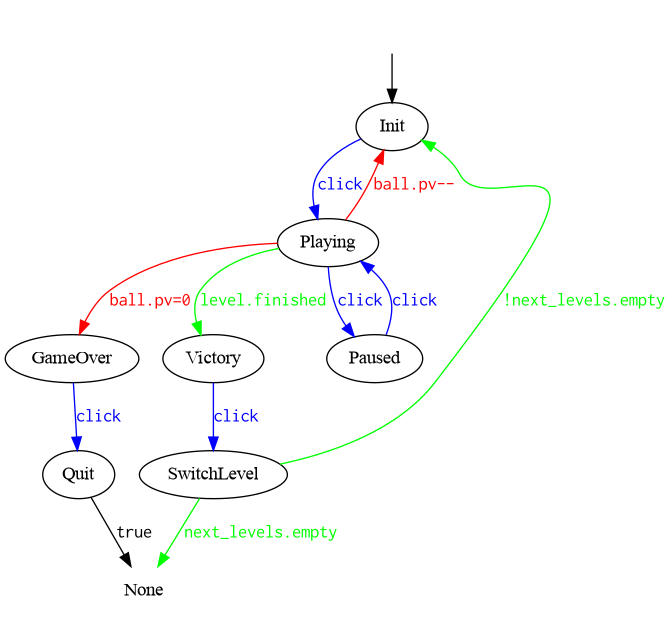
\includegraphics[width=\textwidth]{img/graph.png}
    \caption{Graphe de transition des états de jeu}
    \label{fig:graph}
\end{figure}

\section{Niveaux de jeu}

Initialement, un niveau de jeu était défini en OCaml et chaque brique ajoutée séparément. C'était à la fois verbeux et peu pratique. Nous avons donc "développé" une syntaxe très simple pour définir un niveau textuellement. Chaque type de brique est représenté par un caractère différent et l'air est représenté par un espace. Les bordures sont fixées avec les caractères tiret et barre verticale. Deux exemples de niveaux sont donnés à la figure \ref{fig:level.txt}.

Des exemples de niveaux sont disponibles dans le répertoires \texttt{levels}.

\begin{figure}[ht]
    \begin{minipage}{0.4\textwidth}
        \begin{verbatim}
        |----------------|
        | ############## |
        | ============== |
        | ++++++++++++++ |
        |                |
        |                |
        |                |
        |----------------|
        \end{verbatim}
    \end{minipage}
    \hfill
    \begin{minipage}{0.4\textwidth}
        \begin{verbatim}
        |----------------|
        | @+ + + + + + @ |
        | @ + + + + + +@ |
        | @+ + + + + + @ |
        | @ + + + + + +@ |
        | @@@@@@@@@@@@@@ |
        |                |
        |----------------|
        \end{verbatim}
    \end{minipage}
    \caption{Exemples de niveau}
    \label{fig:level.txt}
\end{figure}

Cette solution a donné une liberté de création qui pose un autre problème. Désormais, les niveaux peuvent avoir différents formats. Afin d'éviter les niveaux débordant de la fenêtre, les dimensiosn de cette dernière sont fonction directe des dimensions du niveau et de la taille des briques.

Ainsi, voici un exemple de ce que permet cette liberté de création:

\begin{figure}[ht]
    \centering
    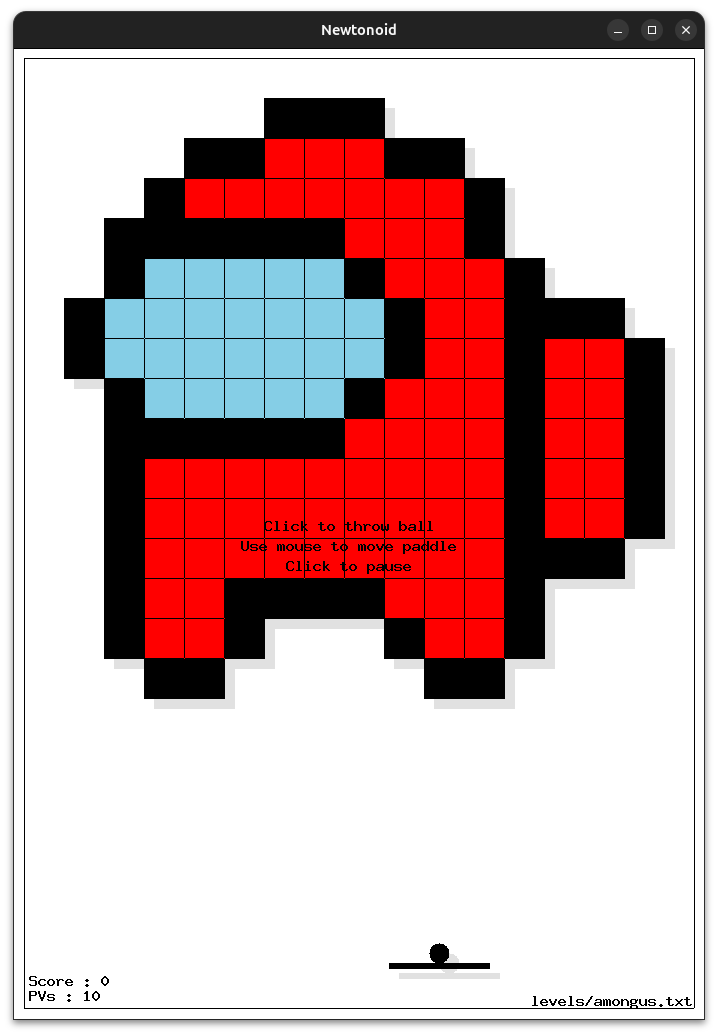
\includegraphics[width=0.5\textwidth]{img/amongus.png}
    \caption{Représentation d'un niveau type Among Us}
    \label{fig:amongus}
\end{figure}

\section{Paramètres}

Nous avons vite compris que la possibilité de changer efficacement les paramètres était cruciale pour le développement et pratique pour le joueur. C'est pourquoi nous avons créé un module \texttt{Params} qui contient tous les paramètres du jeu. L'idée était de paramétrer les autres modules en fonction de \texttt{Params}. Ainsi, chaque module est en partie défini par les paramètres qui lui sont donnés.

Cette paramétrisation des modules permet de diminuer le nombre d'arguments des fonctions ainsi que la présene de valeurs "magiques" dans le code.

Pour faciliter la gestion des paramètres, nous avons développé un "parsing" primitif de fichier ".conf" qui récupère les paramètres du jeu et crée un module \texttt{Params} correspondant. Cette fonctionnalité est implémentée via le foncteur (au sens d'OCaml) \texttt{Params.Make} qui prend en argument un simple module contenant le nom du fichier de configuration et renvoie un module \texttt{Params}.

Des exemples de fichiers de configuration sont disponibles dans le répertoire \texttt{configs}.

\section{Tests}

Les tests unitaires de ce projet sont réalisés avec la bibliothèque \texttt{ppx\_inline\_test}.

Afin d'éviter des paramétrages insensés, à chaque lancement de jeu, \texttt{paramValidator.ml} valide (ou non) les valeurs données par l'utilisateur dans le fichier de configuration. On vérifie par exemple que \texttt{ball\_r > 0}, \texttt{ball\_init\_vy <= ball\_max\_vy} etc.

\section{Contrôles}

\subsection{Démarrer le jeu}

Initialement, le jeu est en pause, la balle collée sur la raquette. Lors du clic du joueur, la balle est propulsée vers le haut et les mises-à-jour commencent à s'effectuer. Le clic change l'état de jeu de \texttt{Init} à \texttt{Playing}.

\subsection{Mettre le jeu en pause}

Le joueur a la possibilité de mettre le jeu en pause en cliquant sur le bouton de sa souris. La fonction \texttt{State.update} change le \texttt{game\_status} de \texttt{Playing} à \texttt{Paused} (et inversement) lorqu'un clic est détecté. Étant donné que la boucle de mise-à-jour continue de tourner mais sans modifier l'état de jeu, il est impératif de rajouter un \texttt{sleep} lors d'un clic, pour éviter de le comptabiliser sur plusieurs frames.

\section{Fin du jeu}

La fin du jeu intervient dans deux cas: le joueur n'a plus de point de vie ( état\texttt{GameOver}), ou le niveau ne contient plus que des briques incassables (état \texttt{Victory}). Dans les deux cas, la mise-à-jour s'arrête et un message de fin s'affiche à l'écran.

\section{Améliorations}

\begin{itemize}
    \item \textbf{Taille du texte:} Les messages de fin de jeu affichés à l'écran sont écrit en petit. Le module \texttt{Graphics} d'OCaml ne possède pas d'implémentation de la fonction \texttt{set\_text\_size} pourtant spécifiée dans l'interface. Il est donc difficile de changer la taille d'écriture.
\end{itemize}

\end{document}